\documentclass[a4paper,11pt]{article}
\usepackage[verbose,a4paper,tmargin=2cm,bmargin=2cm,lmargin=2.5cm,rmargin=2.5cm]{geometry}
\usepackage[utf8]{inputenc}
\usepackage{polski}
\usepackage{amsmath}
\usepackage{amsfonts}
\usepackage{amssymb}
\usepackage{lastpage}
\usepackage{indentfirst}
\usepackage{verbatim}
\usepackage{graphicx}
\usepackage{fancyhdr}
\usepackage{listings}
\usepackage{hyperref} 
\usepackage{xcolor}
\usepackage{tikz}
\usepackage{graphicx} 
\usepackage{float}
\usepackage{verbatim}
\usepackage{graphicx}
\usepackage{fancyhdr}
\usepackage{listings}
\usepackage{color}
\usepackage{pdfpages}
\frenchspacing
\pagestyle{fancyplain}
\fancyhf{}
\renewcommand{\headrulewidth}{0pt}
\renewcommand{\footrulewidth}{0.4pt}
\newcommand{\degree}{\ensuremath{^{\circ}}} 
\fancyfoot[L]{PSI: Justyna Hubert i Karol Podlewski}
\fancyfoot[R]{\thepage\ / \pageref{LastPage}}


\begin{document}

\begin{titlepage}
\begin{center}
\begin{tabular}{rl}
\begin{tabular}{|r|}
\hline \\
\large{\underline{210200~~~~~~~~~~~~~~~~~~~~~~~~~~~~~~~~~~~~~~~~~~} }\\
$^{numer\ indeksu}$\\
\large {\underline{Justyna Hubert~~~~~~~~~~~~~~~~~~~~~~~~~~~~~~} }\\
$^{imie\ i\ nazwisko}$ \\\\ \hline
\end{tabular} 
&
\begin{tabular}{|r|}
\hline \\
\large{\underline{210294~~~~~~~~~~~~~~~~~~~~~~~~~~~~~~~~~~~~~~~~~~} }\\
$^{numer\ indeksu}$\\
\large {\underline{Karol Podlewski~~~~~~~~~~~~~~~~~~~~~~~~~~~~~~} }\\
$^{imie\ i\ nazwisko}$ \\\\ \hline
\end{tabular} 

\end{tabular}
~\\~\\~\\ 
\end{center}
\begin{tabular}{ll}
\LARGE{\textbf{Data}}& \LARGE{2018-10-12}\\
\LARGE{\textbf{Kierunek}}& \LARGE{Informatyka}\\
\LARGE{\textbf{Rok akademicki}}& \LARGE{2018/19} \\
\LARGE{\textbf{Semestr}}& \LARGE{5} \\
\LARGE{\textbf{Specjalizacja}}& \LARGE{IOAD} \\
\LARGE{\textbf{Grupa dziekańska}}& \LARGE{3} \\\\\\\\\\
\end{tabular}

\begin{center}
\textbf{\LARGE{\\~\\Projektowanie Systemów\\Informatycznych\\~\\~\\}}
\end{center}


\begin{center}
\textbf{\Huge{Internetowy sklep z odzieżą:\\~\\ WearIT}} \\~\\
\end{center}

\end{titlepage}
\setcounter{page}{2}

\section {Wprowadzenie}

\subsection {Cel dokumentu}
Celem dokumentu jest przedstawienie projektu systemu informatycznego dla internetowego sklepu z odzieżą WearIT. Dokument ten prezentuje wymagania dotyczące oprogramowania, czyli opisuje funkcjonalność budowanego oprogramowania i warunki, jakie ono musi spełniać. 

\subsection {Zakres produktu}
Projektowany system będzie odpowiedzialny za obsługę składanych zamówień internetowych. Ma on za zadanie usprawnić przebieg pracy pracowników firmy zajmującej się sprzedażą odzieży oraz zautomatyzować proces handlu elektronicznego.


\section {Wymagania}

\subsection {Funkcjonalne}
\begin{itemize}
	\item Rejestracja (tworzenie konta) (możliwość rejestracji za pomocą portali społecznościowych, tj. Facebook, Google).
	\item Logowanie, wylogowywanie.
	\item Dodawanie i usuwanie produktu do koszyka.
	\item Zakup produktów znajdujących się w koszyku.
	\item Sprawdzenie dostępności produktu .
	\item Wyszukiwanie produktów według kategorii, ceny (minimalna, maksymalna), marki, rozmiaru, płci, koloru, kolekcji, stanu (przecenione, nieprzecenione).
	\item Sortowanie listy produktów w kolejności rosnącej i malejącej według ceny, popularności, trafności, daty wydania kolekcji.
	\item Formularz kontaktowy.
	\item Obsługę reklamacji, zwrotów.
	\item Organizację akcji promocyjnych.
	\item Wprowadzanie towaru do systemu.
	\item Zarządzanie stanami magazynowymi.
	\item Przygotowywanie produktów do wysyłki.
\end{itemize} 

\subsection {Niefunkcjonalne}
\begin{itemize}
	\item Certyfikat bezpieczeństwa na stronie internetowej.
	\item Obsługa baz danych.
	\item Wymagane stałe połączenie sieciowe.
	\item Długość nieaktywnej sesji.
	\item Zakupy możliwe tylko po zalogowaniu.
	\item Dodanie do koszyka produktów możliwe także dla klientów niezarejestrowanych/niezalogowanych.
	\item Dostępność systemu dla klientów na urządzeniach moblinych
	\item Maksymalna liczba produktów w koszyku to 25.
	\item Nie można dodać do koszyka produktów niedostępnych.
	\item Darmowa dostawa powyżej 300zł.
\end{itemize}

\subsection {Diagram przypadków użycia}

\begin{figure}[H]
	\centering
		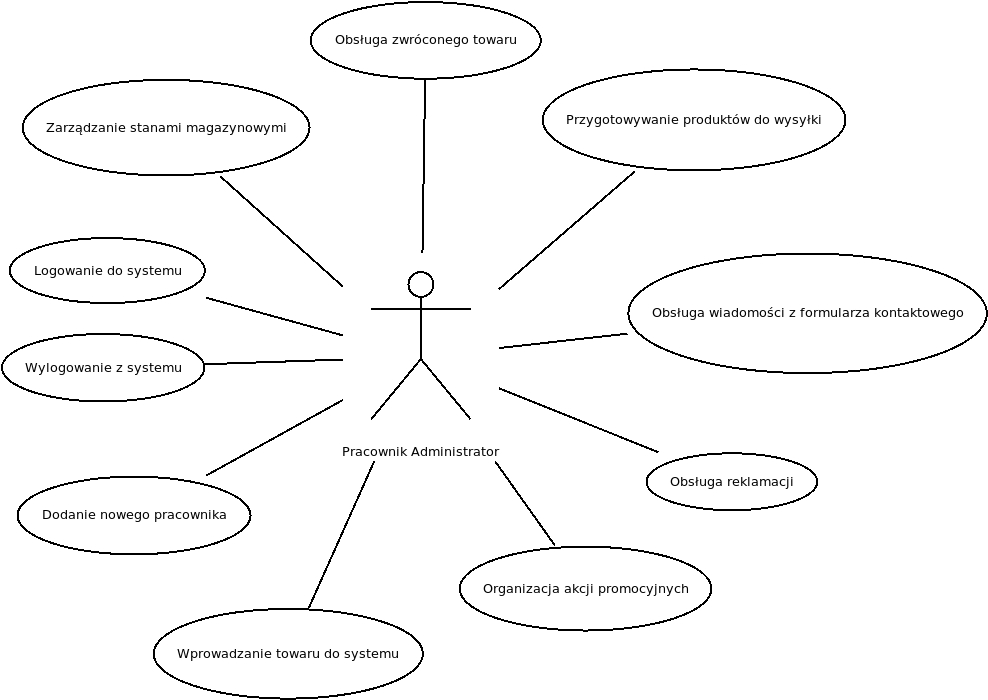
\includegraphics[width=0.8\textwidth]{Diagramy/PrzypadkiUzycia/Admin.jpeg}
	\caption{Diagram przypadku użycia przez administratora.}
\end{figure}
\begin{figure}[H]
	\centering
		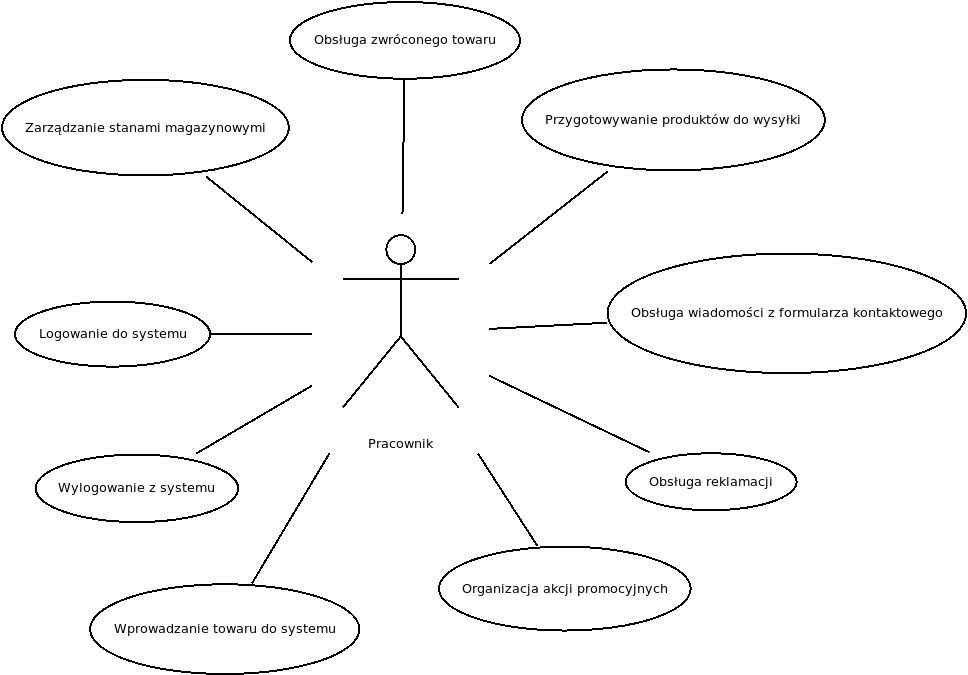
\includegraphics[width=0.8\textwidth]{Diagramy/PrzypadkiUzycia/Pracownik.jpeg}
	\caption{Diagram przypadku użycia przez pracownika.}
\end{figure}
\begin{figure}[H]
	\centering
		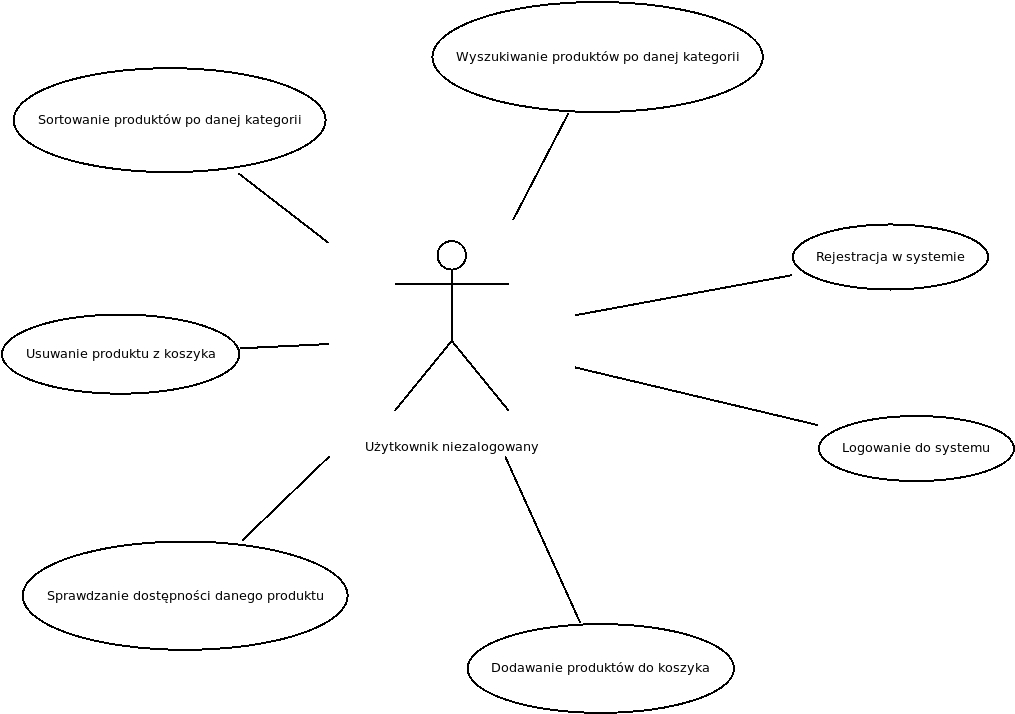
\includegraphics[width=0.8\textwidth]{Diagramy/PrzypadkiUzycia/Niezalogowany.jpeg}
	\caption{Diagram przypadku użycia przez niezalogowanego użytkownika.}
\end{figure}
\begin{figure}[H]
	\centering
		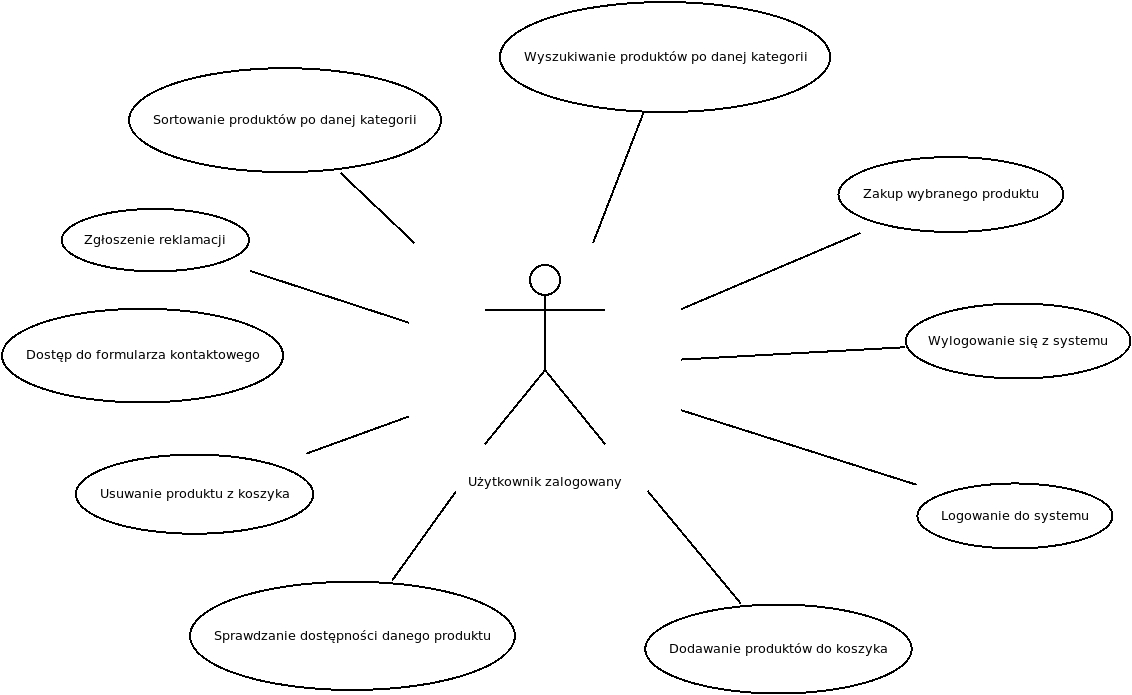
\includegraphics[width=0.8\textwidth]{Diagramy/PrzypadkiUzycia/Zalogowany.jpeg}
	\caption{Diagram przypadku użycia przez zalogowanego użytkownika.}
\end{figure}


\section {Hierarchiczny model funkcji systemu informatycznego}
\subsection {Diagram hierarchii funkcji.}

\begin{figure}[H]
	\centering
		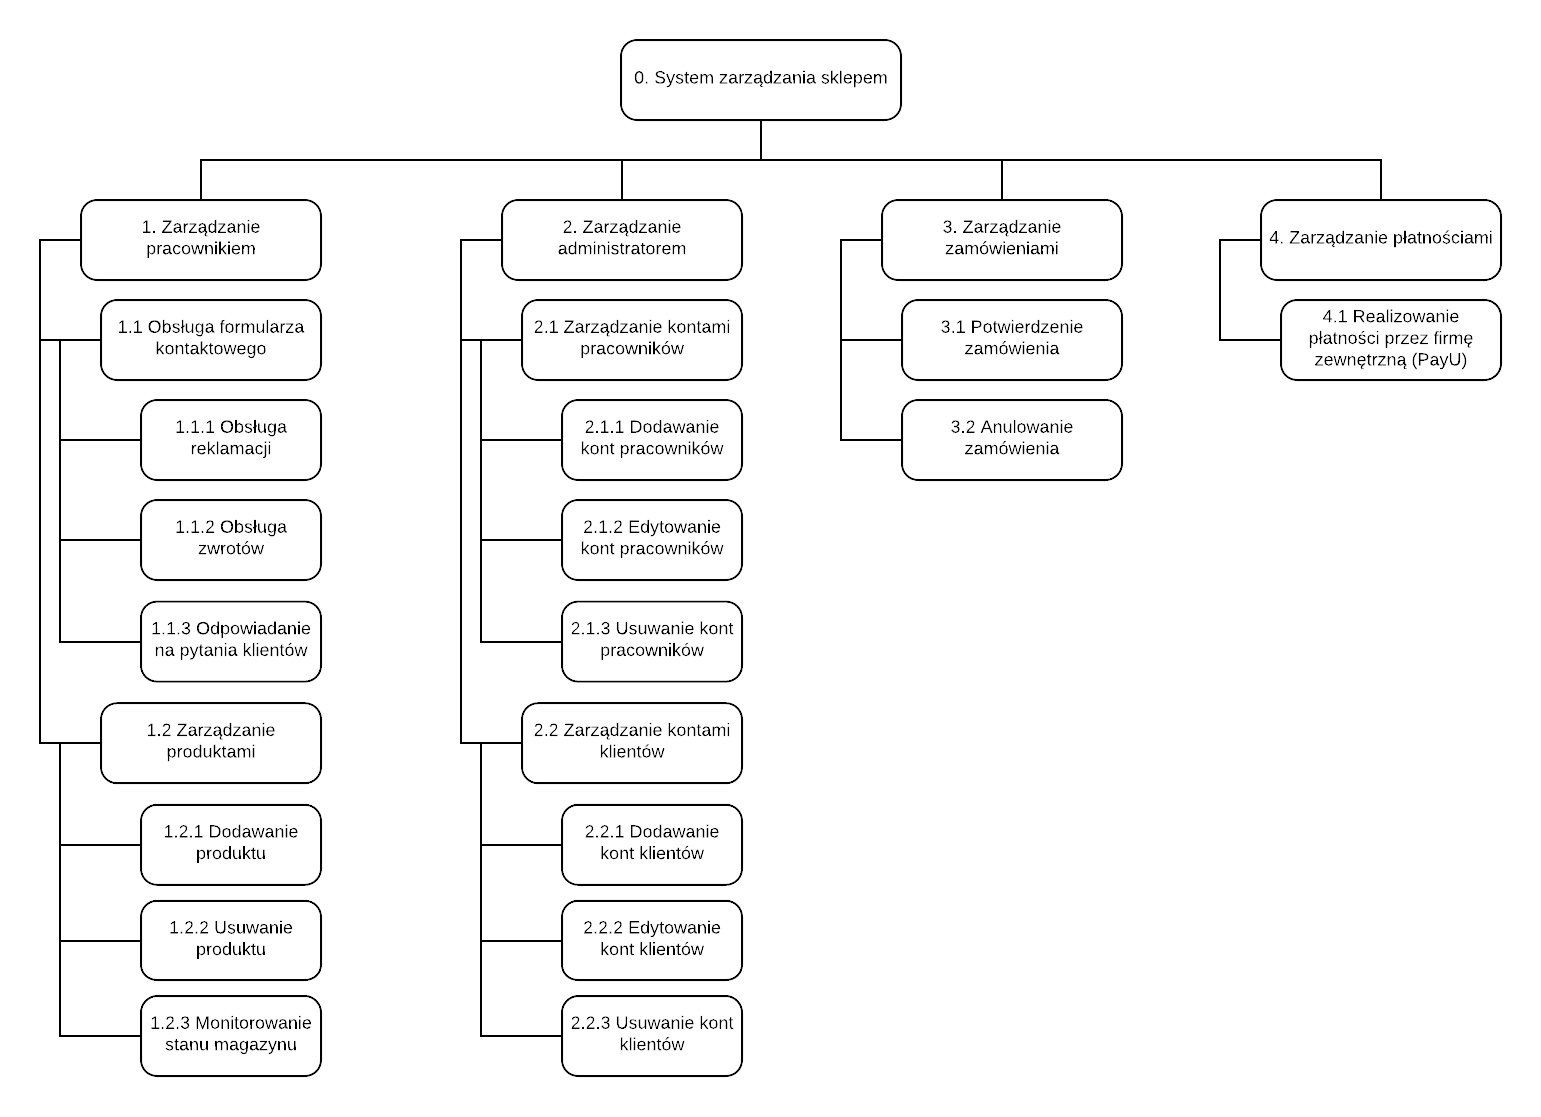
\includegraphics[width=1\textwidth]{Diagramy/HierarchiiFunkcji.png}
	\caption{Diagram hierarchii funkcji.}
\end{figure}

\subsection {Opis diagramu hierarchii funkcji.}
\begin{enumerate}
	\item Obsługa formularza kontaktowego
	\begin{itemize}
		\item Obsługa reklamacji
		\begin{list}{}
			\item Opis: Klient otrzymuje potwierdzenie/odrzucenie reklamacji
			\item Dane wejściowe: Wiadomość od klienta
			\item Wynik: Przy potwierdzeniu reklamacji - zwrot kosztów dla klienta, przy odrzuceniu reklamacji - wiadomość zwrotna dla klienta. 
		\end{list}
		
		\item Obsługa zwrotu
		\begin{list}{}
			\item Opis: Klient otrzymuje potwierdzenie/odrzucenie zwrotu
			\item Dane wejściowe: Wiadomość od klienta
			\item Wynik: Przy potwierdzeniu zwrotu - zwrot kosztów dla klienta, przy odrzuceniu zwrotu - wiadomość zwrotna dla klienta. 
		\end{list}
		
		\item Odpowiadanie na pytania klientów
		\begin{list}{}
			\item Opis: Klient otrzymuje odpowiedź na pytanie
			\item Dane wejściowe: Wiadomość od klienta
			\item Wynik: Wiadomość do klienta z odpowiedzią na jego pytania
		\end{list}
	\end{itemize}
	
	\item Zarządzanie produktami	
	
	\begin{itemize}
		\item Dodanie produktu
		\begin{list}{}
			\item Opis: Dodanie produktu do bazy danych
			\item Dane wejściowe: Dane produktu
			\item Wynik: Produkt zostaje dodany do bazy danych i występuje w systemie
		\end{list}
		
		\item Usunięcie produktu
		\begin{list}{}
			\item Opis: Usunięcie produktu z bazy danych
			\item Dane wejściowe: Dane produktu
			\item Wynik: Produkt zostaje usunięty z bazy danych i nie występuje w systemie
		\end{list}
		
		\item Monitorowanie stanu magazynu
		\begin{list}{}
			\item Opis: Aktualizacja dostępności produktów w systemie
			\item Dane wejściowe: Dane produktu
			\item Wynik: Produkt zostaje oznaczony jako dostępny/niedostępny 
		\end{list}
	\end{itemize}

	\item Zarządzanie kontami pracowników
	\begin{itemize}
	
		\item Dodawanie kont pracowników
		\begin{list}{}
			\item Opis: Dodanie pracownika do systemu
			\item Dane wejściowe: Dane pracownika
			\item Wynik: Pracownik znajduje się bazie danych 
		\end{list}
		
		\item Edytowanie kont pracowników
		\begin{list}{}
			\item Opis: Edycja konta pracownika
			\item Dane wejściowe: Dane pracownika
			\item Wynik: Zmodyfikowane dane pracownika znajdują się w systemie
		\end{list}
		
		\item Usuwanie kont pracowników
		\begin{list}{}
			\item Opis: Usunięcie konta pracownika
			\item Dane wejściowe: Dane pracownika
			\item Wynik: Konto pracownika nie znajduje się w bazie danych
		\end{list}
		
	\end{itemize}
	
	\item Zarządzanie kontami klientów
	\begin{itemize}
		\item Dodawanie kont klientów
		\begin{list}{}
			\item Opis: Dodanie klienta do systemu
			\item Dane wejściowe: Dane klienta
			\item Wynik: Klient znajduje się bazie danych 
		\end{list}
		
		\item Edytowanie kont klientów
		\begin{list}{}
			\item Opis: Edycja konta klienta
			\item Dane wejściowe: Dane klienta
			\item Wynik: Zmodyfikowane dane klienta znajdują się w systemie
		\end{list}
		
		\item Usuwanie kont klientów
		\begin{list}{}
			\item Opis: Usunięcie konta klienta
			\item Dane wejściowe: Dane klienta
			\item Wynik: Konto klienta nie znajduje się w bazie danych
		\end{list}
	
	\end{itemize}
	
	\item Zarządzanie zamówieniami
		\begin{itemize}
		\item Potwierdzenie zamówienia
		\begin{list}{}
			\item Opis: Przyjęcie zamówienia do realizacji
			\item Dane wejściowe: Dane zamówienia
			\item Wynik: Wysłana zostaje informacja do klienta, że jego zamówienie będzie realizowane
		\end{list}
		
		\item Anulowanie zamówienia
		\begin{list}{}
			\item Opis: Nieprzyjęcie zamówienia do realizacji
			\item Dane wejściowe: Dane zamówienia
			\item Wynik: Wysłana zostaje informacja do klienta, że jego zamówienie nie będzie realizowane
		\end{list}
		\end{itemize}
\end{enumerate}

\section {Diagram kontekstowy DFD0}

\begin{figure}[H]
	\centering
		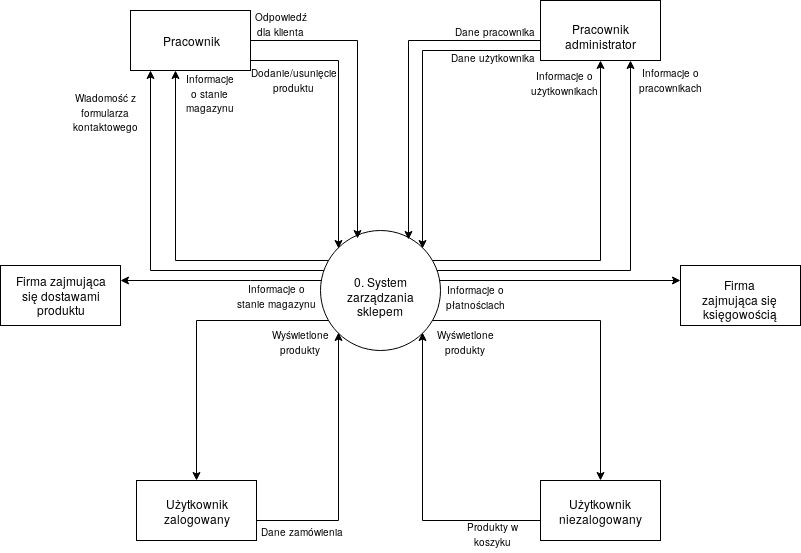
\includegraphics[width=0.8\textwidth]{Diagramy/DFD0.png}
	\caption{Diagram kontekstowy DFD0.}
\end{figure}

\section {Projekt struktury funkcjonalnej systemu.}

\begin{figure}[H]
	\centering
		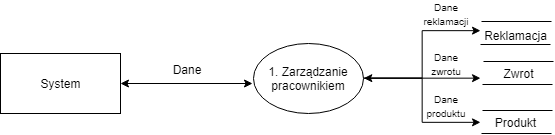
\includegraphics[width=0.8\textwidth]{Diagramy/DFD0-DFD1.png}
	\caption{Diagram DFD zarządzania pracownikiem.}
\end{figure}

\begin{figure}[H]
	\centering
		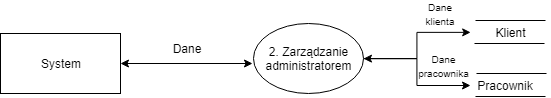
\includegraphics[width=0.8\textwidth]{Diagramy/DFD0-DFD2.png}
	\caption{Diagram DFD zarządzania administratorem.}
\end{figure}

\begin{figure}[H]
	\centering
		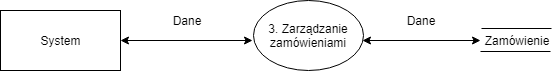
\includegraphics[width=0.8\textwidth]{Diagramy/DFD0-DFD3.png}
	\caption{Diagram DFD zarządzania zamówieniami.}
\end{figure}

\begin{figure}[H]
	\centering
		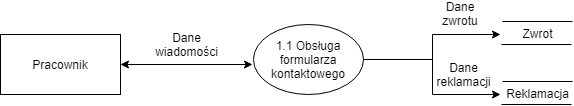
\includegraphics[width=0.8\textwidth]{Diagramy/DFD0-DFD11.png}
	\caption{Diagram DFD obsługi formularza kontaktowego.}
\end{figure}


\begin{figure}[H]
	\centering
		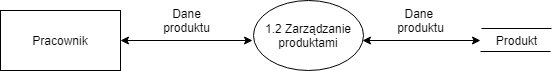
\includegraphics[width=0.8\textwidth]{Diagramy/DFD0-DFD12.png}
	\caption{Diagram DFD zarządzania produktami.}
\end{figure}

\begin{figure}[H]
	\centering
		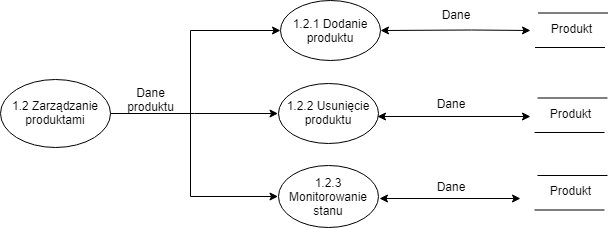
\includegraphics[width=0.8\textwidth]{Diagramy/DFD0-pracownik-produkt.png}
	\caption{Diagram DFD zarządzania produktami z niższego poziomu.}
\end{figure}

\begin{figure}[H]
	\centering
		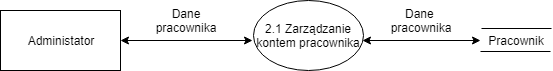
\includegraphics[width=0.8\textwidth]{Diagramy/DFD0-DFD22.png}
	\caption{Diagram DFD zarządzania kontem pracownika.}
\end{figure}

\begin{figure}[H]
	\centering
		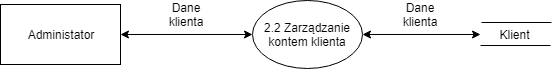
\includegraphics[width=0.8\textwidth]{Diagramy/DFD0-DFD21.png}
	\caption{Diagram DFD zarządzania kontem klienta.}
\end{figure}

\begin{figure}[H]
	\centering
		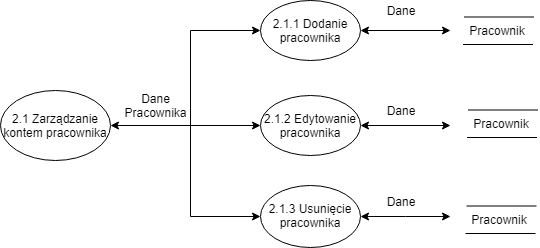
\includegraphics[width=0.8\textwidth]{Diagramy/DFD0-admin-pracownik.png}
	\caption{Diagram DFD zarządzania kontem pracownika z niższego poziomu.}
\end{figure}

\begin{figure}[H]
	\centering
		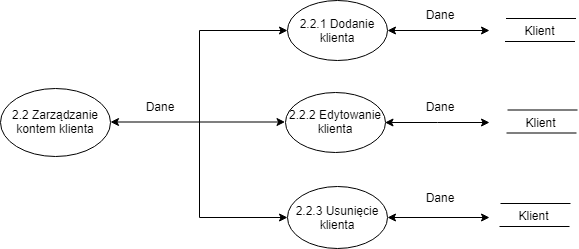
\includegraphics[width=0.8\textwidth]{Diagramy/DFD0-admin-klient.png}
	\caption{Diagram DFD zarządzania kontem klienta z niższego poziomu.}
\end{figure}

\begin{figure}[H]
	\centering
		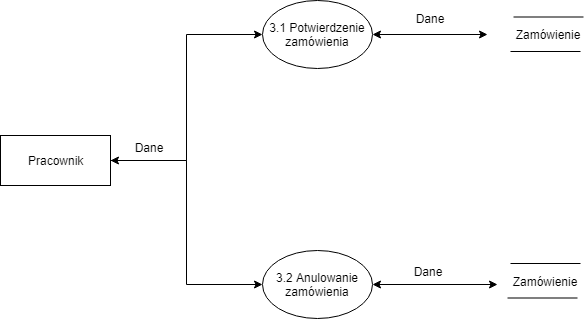
\includegraphics[width=0.8\textwidth]{Diagramy/DFD0-DFD-Zamowienie.png}
	\caption{Diagram DFD zamówień.}
\end{figure}

\section {Projekt struktury informacyjnej.}
\subsection {Model Konceptualny – Diagram ERD.}

\begin{figure}[H]
	\centering
		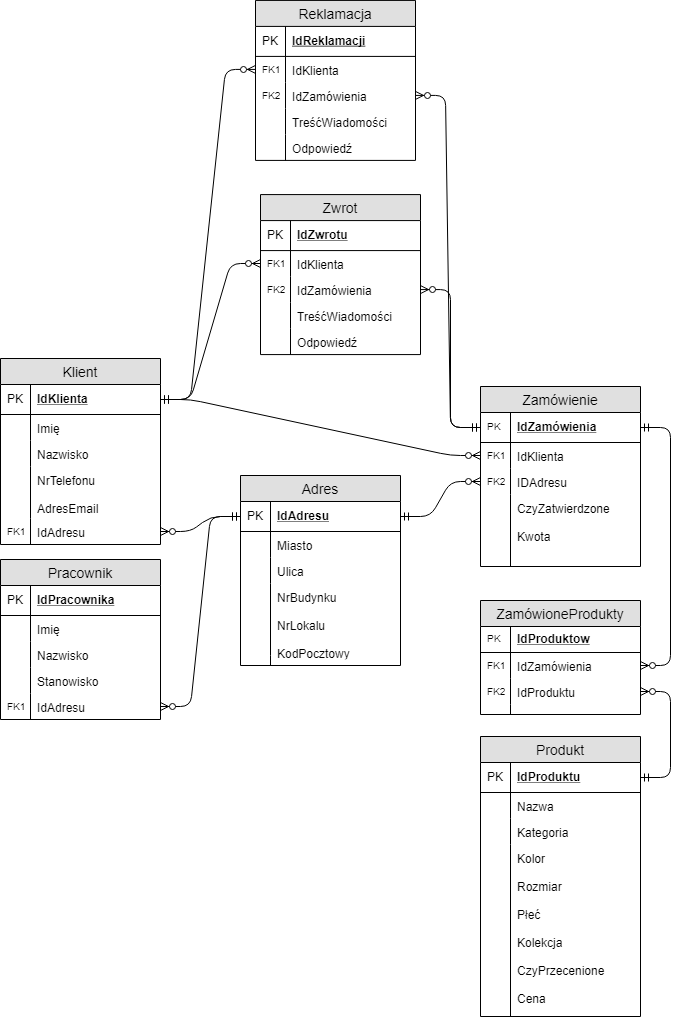
\includegraphics[width=0.9\textwidth]{Diagramy/DFD0-Baza-Danych.png}
	\caption{Diagram ERD.}
\end{figure}

\subsection {Model implementacyjny – Diagram Klas.}
\begin{figure}[H]
	\centering
		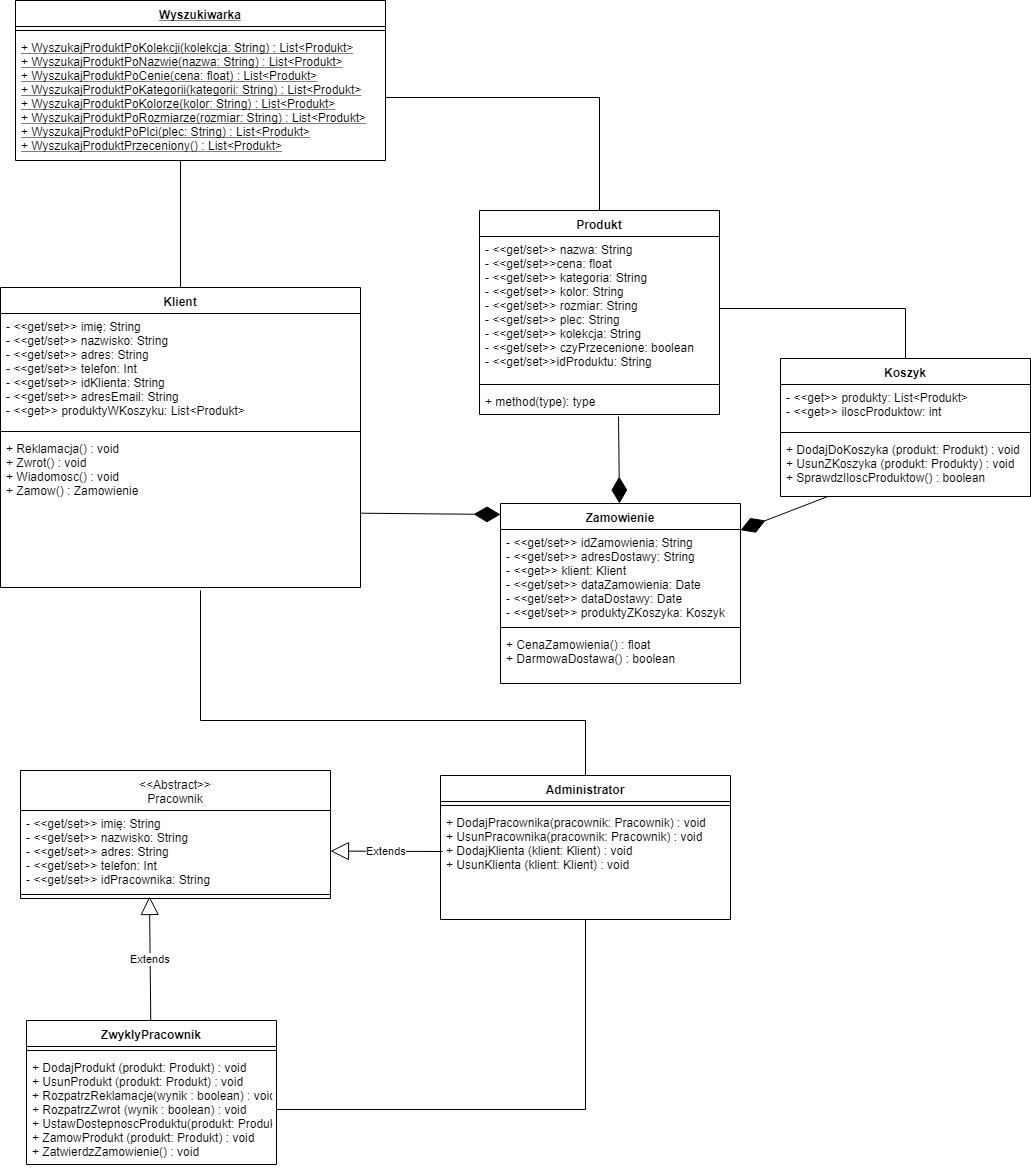
\includegraphics[width=1\textwidth]{Diagramy/DFD0-Diagram-UML.png}
	\caption{Diagram klas.}
\end{figure}

\section {Słownik danych}
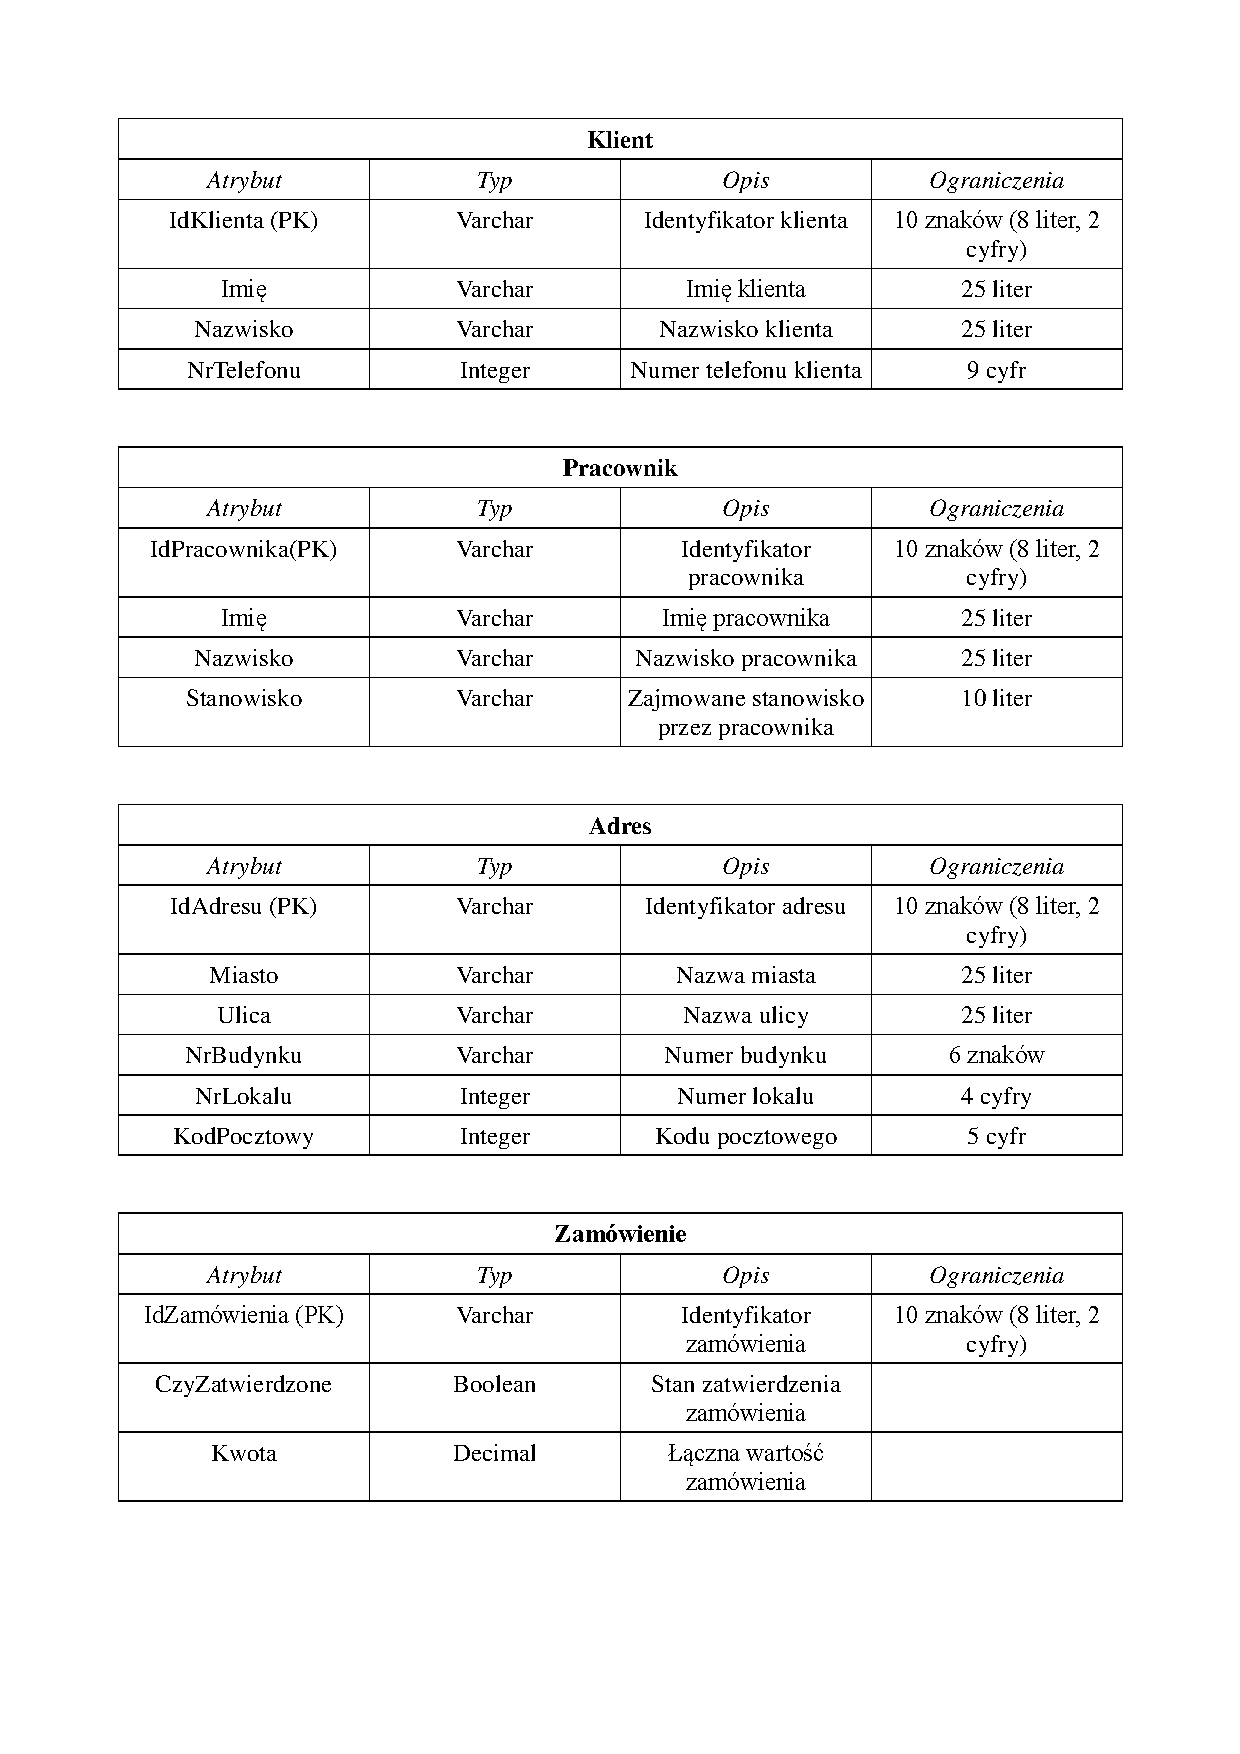
\includepdf[pages=-]{Slowniczek.pdf}

\section {Projekt interfejsu użytkownika.}
\subsection {Koncepcja Interfejsu użytkownika.}
Interfejs użytkownika zostanie stworzony przy użyciu technologii html i css. Interfejs będzie przejrzysty oraz intuicyjny. 

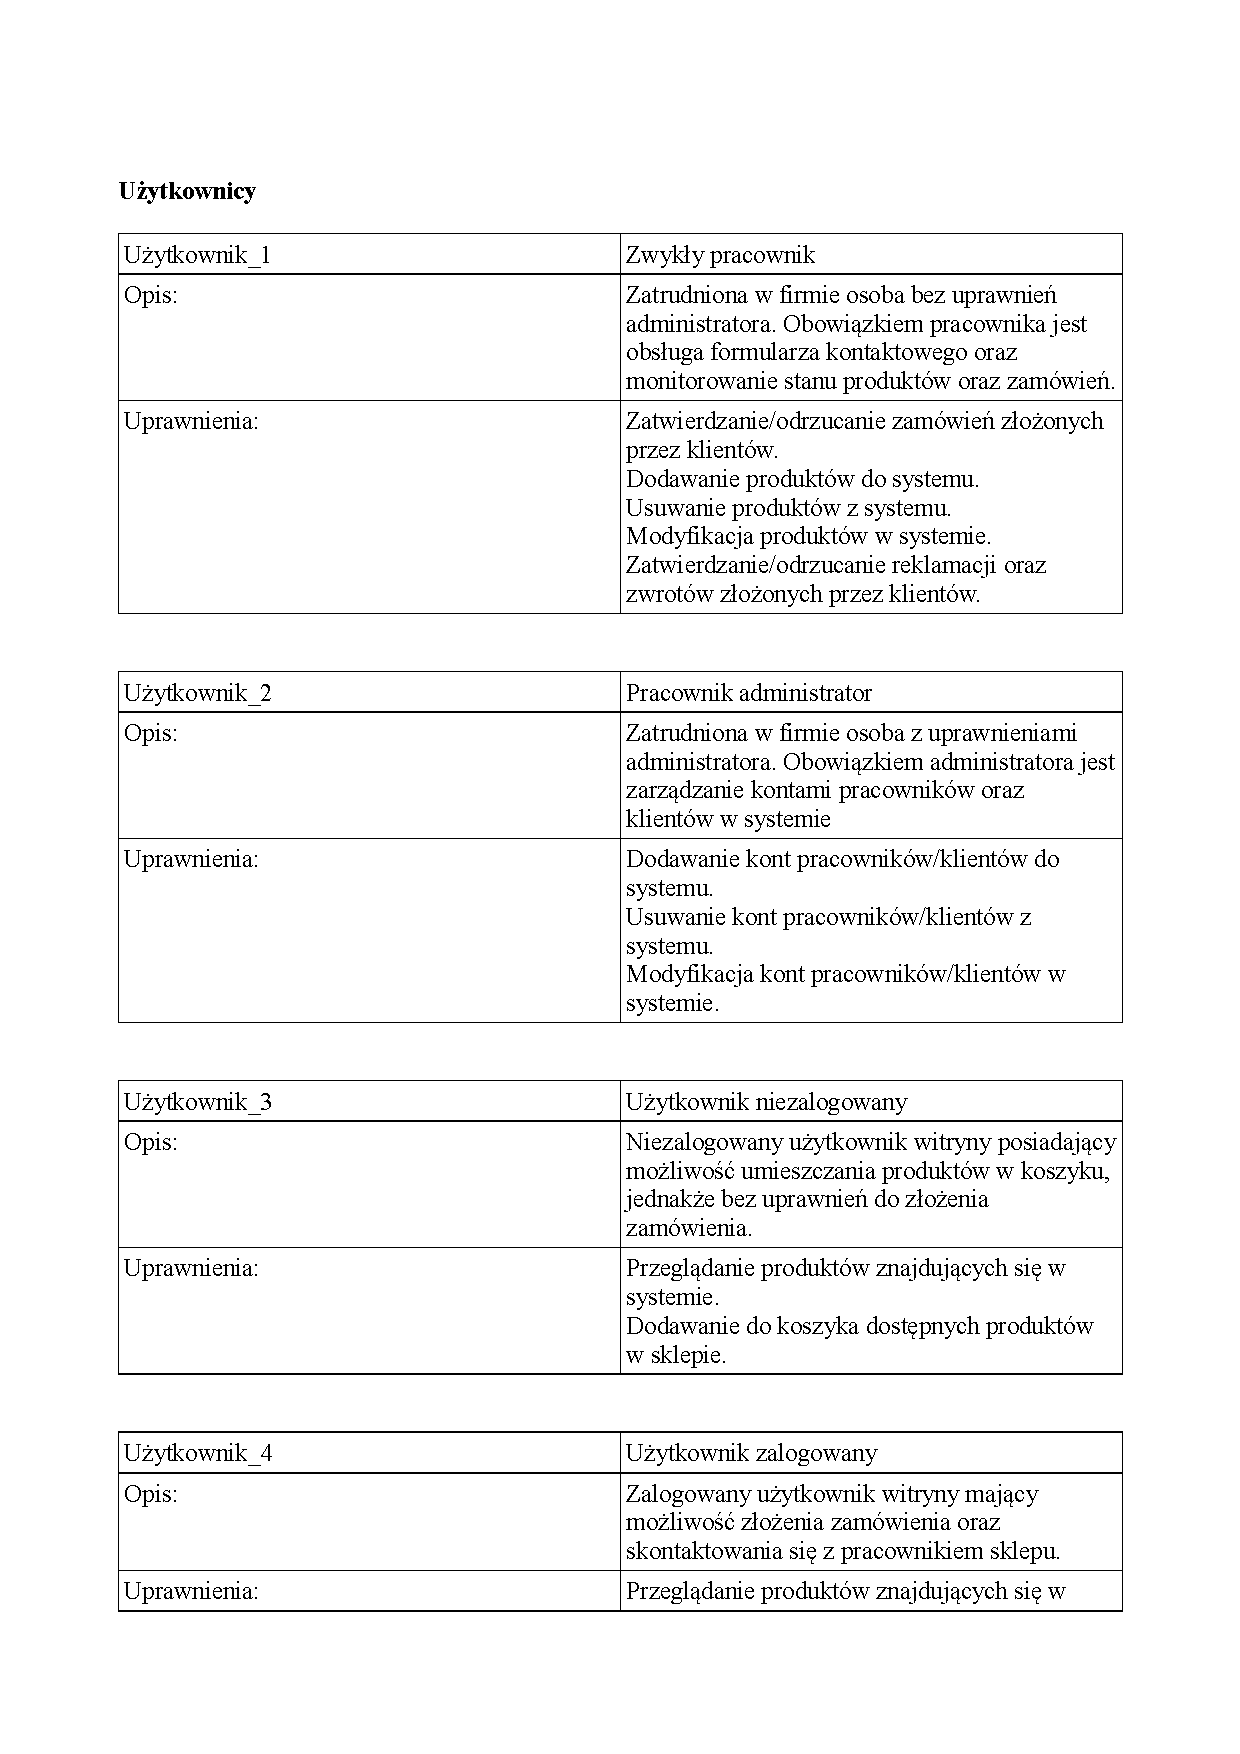
\includepdf[pages=-]{Uzytkownicy.pdf}

\section {Struktura techniczno-przestrzenna systemu.}
System będzie dostępny z poziomu każdej przeglądarki internetowej (Internet Explorer także). System, w zależności od rodzaju otrzymanych uprawnień, będzie umożliwiał różne, wyżej wymienione funkcje. Logika systemu zostanie wykonana w języku Java. 

\end{document}

